\documentclass[10pt]{article}
\usepackage[T1]{fontenc}
\usepackage{lmodern}
\usepackage{mathtools}
\usepackage{booktabs}
\usepackage{adjustbox}
\usepackage[left=1.5cm, right=2cm, top=1.5cm, bottom=2cm]{geometry}
\usepackage{tikz}
\usepackage{pgfplots}
\pgfplotsset{compat=1.18}
\usetikzlibrary{arrows.meta,positioning,calc}
\setlength\parindent{0pt}
\title{g7 5 - No Protection - Custom Algorithm - Descending}
\date{}
\author{}

\begin{document}
\maketitle
\section*{Topology}
\begin{center}\begin{adjustbox}{max width=\linewidth}
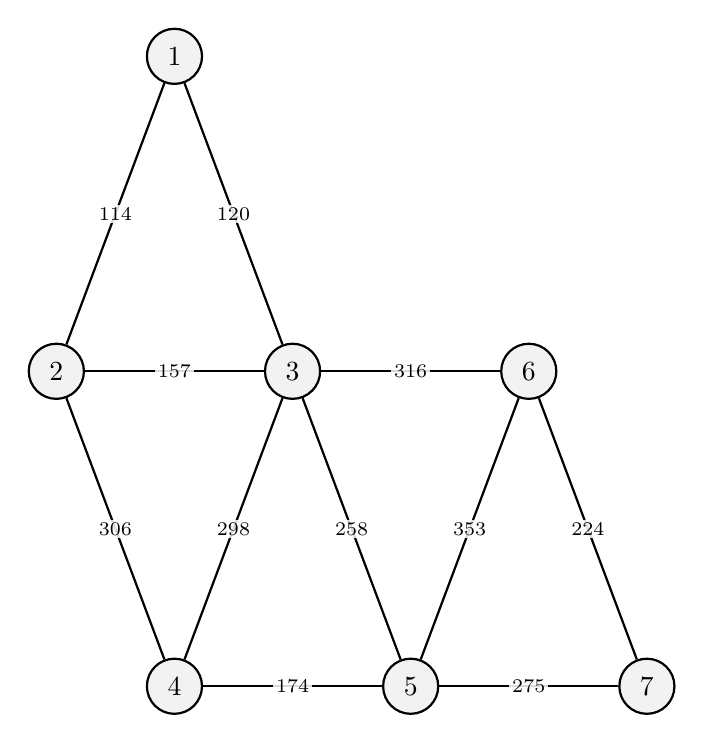
\begin{tikzpicture}[baseline, >={Stealth[length=2mm]},
  netnode/.style={circle, draw, thick, fill=gray!10, minimum size=7mm, inner sep=1pt},
  link/.style={thick},
  linklabel/.style={font=\scriptsize, inner sep=1pt, fill=white, fill opacity=0.85, text opacity=1}]
\node[netnode] (S1) at (1.500,8.000) {1};
\node[netnode] (S2) at (0.000,4.000) {2};
\node[netnode] (S3) at (3.000,4.000) {3};
\node[netnode] (S4) at (1.500,0.000) {4};
\node[netnode] (S5) at (4.500,0.000) {5};
\node[netnode] (S6) at (6.000,4.000) {6};
\node[netnode] (S7) at (7.500,0.000) {7};
\draw[link] (S1) to node[linklabel] {114} (S2);
\draw[link] (S1) to node[linklabel] {120} (S3);
\draw[link] (S2) to node[linklabel] {157} (S3);
\draw[link] (S2) to node[linklabel] {306} (S4);
\draw[link] (S3) to node[linklabel] {298} (S4);
\draw[link] (S3) to node[linklabel] {258} (S5);
\draw[link] (S3) to node[linklabel] {316} (S6);
\draw[link] (S4) to node[linklabel] {174} (S5);
\draw[link] (S5) to node[linklabel] {353} (S6);
\draw[link] (S5) to node[linklabel] {275} (S7);
\draw[link] (S6) to node[linklabel] {224} (S7);
\end{tikzpicture}
\end{adjustbox}\end{center}
\section*{Performance Parameters}
\begin{center}\begin{tabular}{lr}
\toprule
Highest link load & 848 Gb/s \\
Highest used FSU & 186 / 320 \\
Total used FSUs & 207 \\
Transponder cost & 113.5 \\
\midrule
SC-DP-QPSK transponders & 8 \\
SC-DP-16QAM transponders & 23 \\
DP-16QAM transponders & 15 \\
\bottomrule
\end{tabular}\end{center}
\clearpage
\section*{Link Load Map}
\begin{center}\begin{adjustbox}{max width=\linewidth}
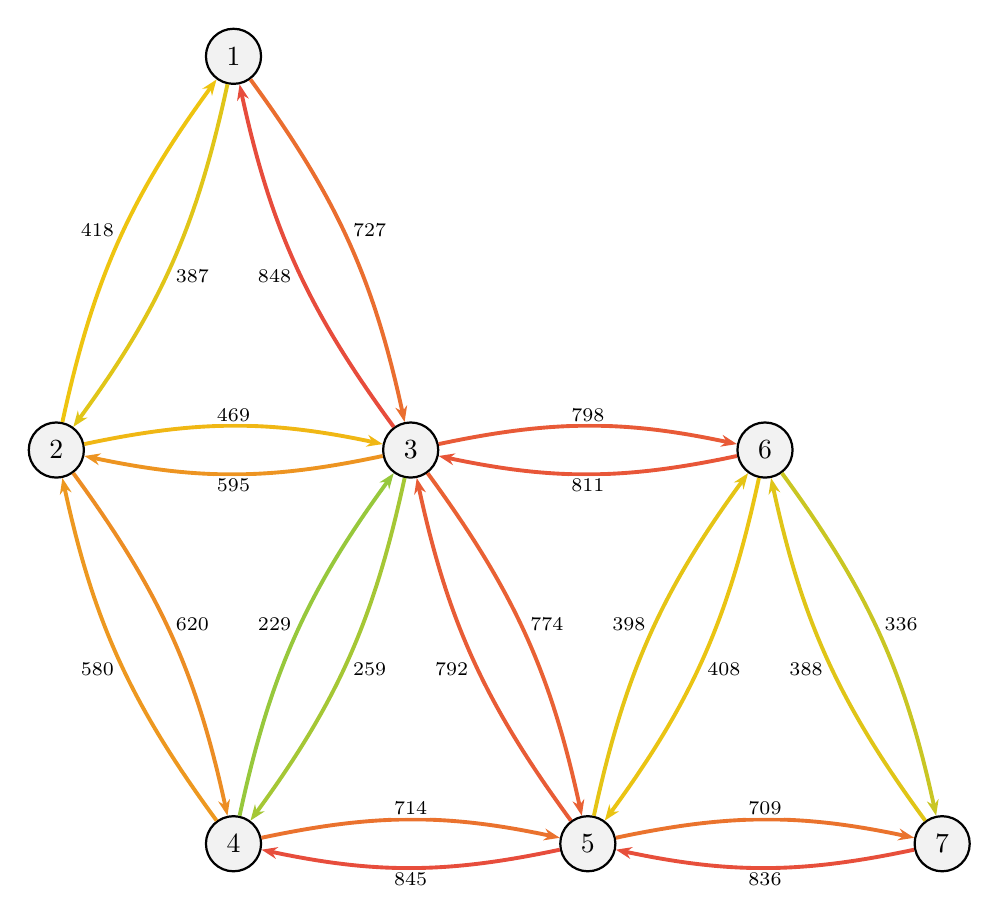
\begin{tikzpicture}[baseline, >={Stealth[length=2mm]},
  netnode/.style={circle, draw, thick, fill=gray!10, minimum size=7mm, inner sep=1pt},
  link/.style={line width=1.4pt},
  linklabel/.style={font=\scriptsize, inner sep=1pt, fill=white, fill opacity=0.85, text opacity=1}]
\node[netnode] (S1) at (2.250,10.000) {1};
\node[netnode] (S2) at (0.000,5.000) {2};
\node[netnode] (S3) at (4.500,5.000) {3};
\node[netnode] (S4) at (2.250,0.000) {4};
\node[netnode] (S5) at (6.750,0.000) {5};
\node[netnode] (S6) at (9.000,5.000) {6};
\node[netnode] (S7) at (11.250,0.000) {7};
\draw[link, ->, draw={rgb,255:red,224;green,197;blue,24}] (S1) to[bend left=12] node[linklabel, auto] {387} (S2);
\draw[link, ->, draw={rgb,255:red,234;green,110;blue,47}] (S1) to[bend left=12] node[linklabel, auto] {727} (S3);
\draw[link, ->, draw={rgb,255:red,238;green,196;blue,16}] (S2) to[bend left=12] node[linklabel, auto] {418} (S1);
\draw[link, ->, draw={rgb,255:red,240;green,183;blue,20}] (S2) to[bend left=12] node[linklabel, auto] {469} (S3);
\draw[link, ->, draw={rgb,255:red,236;green,141;blue,36}] (S2) to[bend left=12] node[linklabel, auto] {620} (S4);
\draw[link, ->, draw={rgb,255:red,231;green,76;blue,60}] (S3) to[bend left=12] node[linklabel, auto] {848} (S1);
\draw[link, ->, draw={rgb,255:red,237;green,148;blue,33}] (S3) to[bend left=12] node[linklabel, auto] {595} (S2);
\draw[link, ->, draw={rgb,255:red,165;green,199;blue,53}] (S3) to[bend left=12] node[linklabel, auto] {259} (S4);
\draw[link, ->, draw={rgb,255:red,233;green,97;blue,52}] (S3) to[bend left=12] node[linklabel, auto] {774} (S5);
\draw[link, ->, draw={rgb,255:red,232;green,90;blue,55}] (S3) to[bend left=12] node[linklabel, auto] {798} (S6);
\draw[link, ->, draw={rgb,255:red,237;green,152;blue,32}] (S4) to[bend left=12] node[linklabel, auto] {580} (S2);
\draw[link, ->, draw={rgb,255:red,151;green,200;blue,60}] (S4) to[bend left=12] node[linklabel, auto] {229} (S3);
\draw[link, ->, draw={rgb,255:red,234;green,114;blue,46}] (S4) to[bend left=12] node[linklabel, auto] {714} (S5);
\draw[link, ->, draw={rgb,255:red,232;green,92;blue,54}] (S5) to[bend left=12] node[linklabel, auto] {792} (S3);
\draw[link, ->, draw={rgb,255:red,231;green,77;blue,60}] (S5) to[bend left=12] node[linklabel, auto] {845} (S4);
\draw[link, ->, draw={rgb,255:red,229;green,196;blue,21}] (S5) to[bend left=12] node[linklabel, auto] {398} (S6);
\draw[link, ->, draw={rgb,255:red,234;green,115;blue,45}] (S5) to[bend left=12] node[linklabel, auto] {709} (S7);
\draw[link, ->, draw={rgb,255:red,232;green,86;blue,56}] (S6) to[bend left=12] node[linklabel, auto] {811} (S3);
\draw[link, ->, draw={rgb,255:red,234;green,196;blue,19}] (S6) to[bend left=12] node[linklabel, auto] {408} (S5);
\draw[link, ->, draw={rgb,255:red,201;green,198;blue,35}] (S6) to[bend left=12] node[linklabel, auto] {336} (S7);
\draw[link, ->, draw={rgb,255:red,231;green,79;blue,59}] (S7) to[bend left=12] node[linklabel, auto] {836} (S5);
\draw[link, ->, draw={rgb,255:red,224;green,197;blue,23}] (S7) to[bend left=12] node[linklabel, auto] {388} (S6);
\end{tikzpicture}
\end{adjustbox}\end{center}
\begin{center}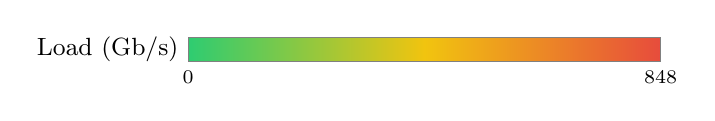
\begin{tikzpicture}
\definecolor{scalelow}{RGB}{46,204,113}\definecolor{scalemid}{RGB}{241,196,15}\definecolor{scalehigh}{RGB}{231,76,60}
\shade[left color=scalelow, right color=scalemid] (0,0) rectangle (3,0.3);
\shade[left color=scalemid, right color=scalehigh] (3,0) rectangle (6,0.3);
\draw[gray] (0,0) rectangle (6,0.3);
\node[below, font=\scriptsize] at (0,0) {0};
\node[below, font=\scriptsize] at (6,0) {848};
\node[left, font=\small] at (0,0.15) {Load (Gb/s)};
\end{tikzpicture}\end{center}
\section*{Link Load Distribution}

\begin{center}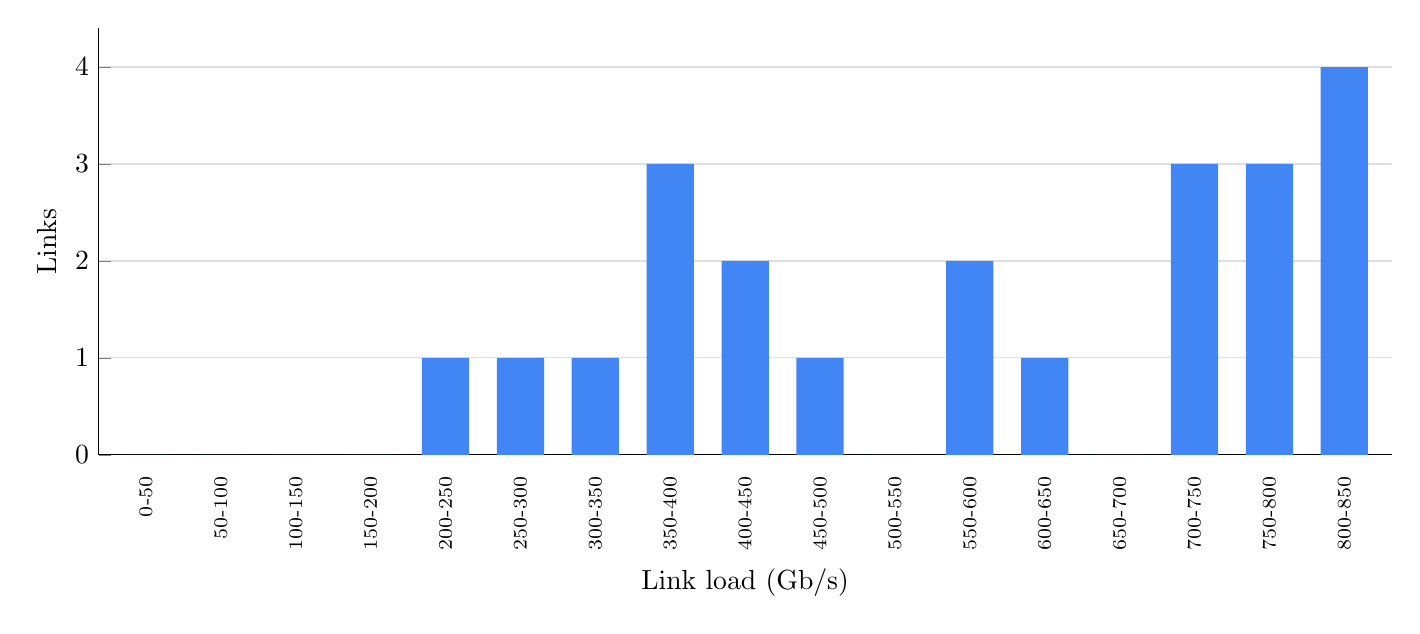
\begin{tikzpicture}
\begin{axis}[
  ybar, bar width=0.600cm, width=18.000cm, height=7cm,
  ymin=0, ymajorgrids, grid style={gray!25}, axis lines*=left,
  enlarge x limits={abs=0.600cm}, xtick=data, major x tick style={draw=none},
  x tick label style={rotate=90, font=\scriptsize, /pgf/number format/1000 sep=},
  legend style={at={(0.5,-0.3)}, anchor=north, legend columns=-1, draw=none},
  ylabel={Links},
  xlabel={Link load (Gb/s)},
  symbolic x coords={0-50,50-100,100-150,150-200,200-250,250-300,300-350,350-400,400-450,450-500,500-550,550-600,600-650,650-700,700-750,750-800,800-850}]
\addplot[fill={rgb,255:red,66;green,133;blue,244}, draw=none] coordinates {(0-50,0.000) (50-100,0.000) (100-150,0.000) (150-200,0.000) (200-250,1.000) (250-300,1.000) (300-350,1.000) (350-400,3.000) (400-450,2.000) (450-500,1.000) (500-550,0.000) (550-600,2.000) (600-650,1.000) (650-700,0.000) (700-750,3.000) (750-800,3.000) (800-850,4.000) };
\end{axis}
\end{tikzpicture}\end{center}
\clearpage
\section*{Spectrum Occupancy}
\begin{center}\begin{adjustbox}{max width=\linewidth}
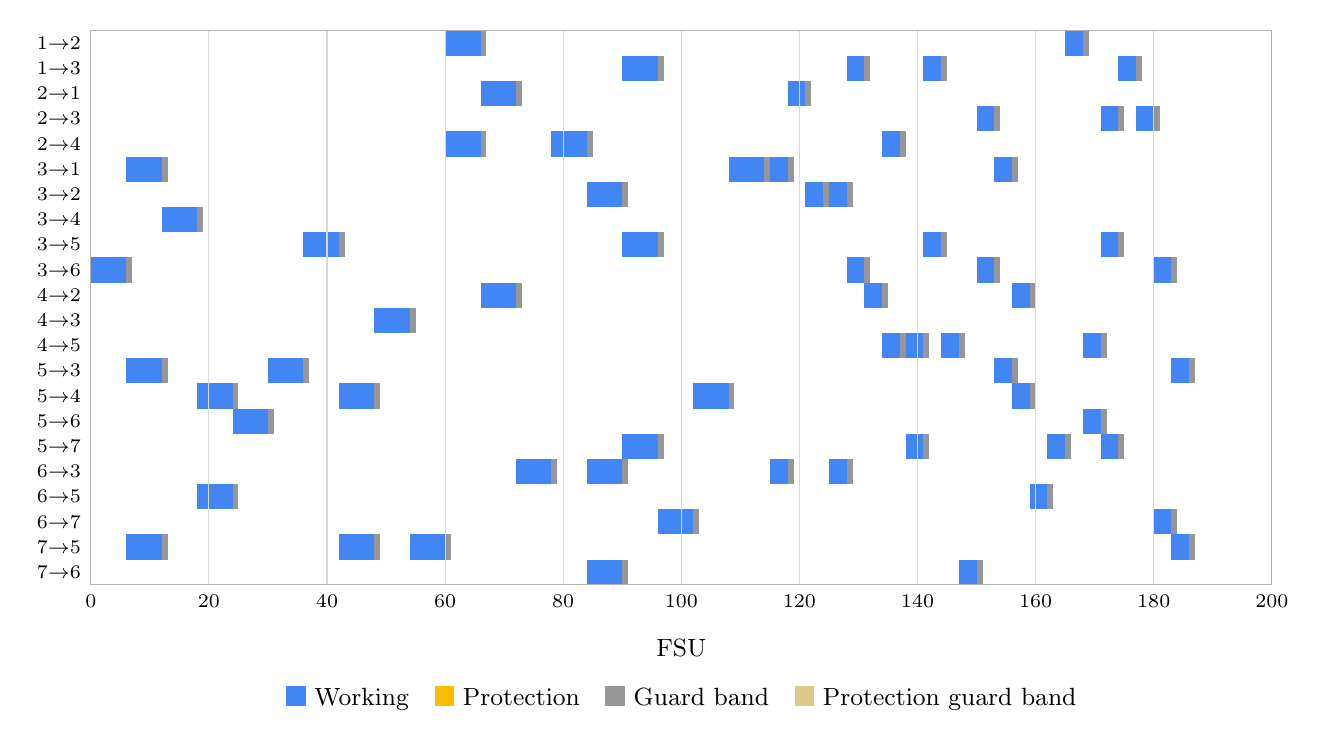
\begin{tikzpicture}[x=0.0750cm, y=-0.32cm]
\fill[fill={rgb,255:red,66;green,133;blue,244}] (60,0) rectangle (66,1);
\fill[fill={rgb,255:red,150;green,150;blue,150}] (66,0) rectangle (67,1);
\fill[fill={rgb,255:red,66;green,133;blue,244}] (165,0) rectangle (168,1);
\fill[fill={rgb,255:red,150;green,150;blue,150}] (168,0) rectangle (169,1);
\node[left, font=\scriptsize] at (0,0.5) {1\(\to\)2};
\fill[fill={rgb,255:red,66;green,133;blue,244}] (90,1) rectangle (96,2);
\fill[fill={rgb,255:red,150;green,150;blue,150}] (96,1) rectangle (97,2);
\fill[fill={rgb,255:red,66;green,133;blue,244}] (128,1) rectangle (131,2);
\fill[fill={rgb,255:red,150;green,150;blue,150}] (131,1) rectangle (132,2);
\fill[fill={rgb,255:red,66;green,133;blue,244}] (141,1) rectangle (144,2);
\fill[fill={rgb,255:red,150;green,150;blue,150}] (144,1) rectangle (145,2);
\fill[fill={rgb,255:red,66;green,133;blue,244}] (174,1) rectangle (177,2);
\fill[fill={rgb,255:red,150;green,150;blue,150}] (177,1) rectangle (178,2);
\node[left, font=\scriptsize] at (0,1.5) {1\(\to\)3};
\fill[fill={rgb,255:red,66;green,133;blue,244}] (66,2) rectangle (72,3);
\fill[fill={rgb,255:red,150;green,150;blue,150}] (72,2) rectangle (73,3);
\fill[fill={rgb,255:red,66;green,133;blue,244}] (118,2) rectangle (121,3);
\fill[fill={rgb,255:red,150;green,150;blue,150}] (121,2) rectangle (122,3);
\node[left, font=\scriptsize] at (0,2.5) {2\(\to\)1};
\fill[fill={rgb,255:red,66;green,133;blue,244}] (150,3) rectangle (153,4);
\fill[fill={rgb,255:red,150;green,150;blue,150}] (153,3) rectangle (154,4);
\fill[fill={rgb,255:red,66;green,133;blue,244}] (171,3) rectangle (174,4);
\fill[fill={rgb,255:red,150;green,150;blue,150}] (174,3) rectangle (175,4);
\fill[fill={rgb,255:red,66;green,133;blue,244}] (177,3) rectangle (180,4);
\fill[fill={rgb,255:red,150;green,150;blue,150}] (180,3) rectangle (181,4);
\node[left, font=\scriptsize] at (0,3.5) {2\(\to\)3};
\fill[fill={rgb,255:red,66;green,133;blue,244}] (60,4) rectangle (66,5);
\fill[fill={rgb,255:red,150;green,150;blue,150}] (66,4) rectangle (67,5);
\fill[fill={rgb,255:red,66;green,133;blue,244}] (78,4) rectangle (84,5);
\fill[fill={rgb,255:red,150;green,150;blue,150}] (84,4) rectangle (85,5);
\fill[fill={rgb,255:red,66;green,133;blue,244}] (134,4) rectangle (137,5);
\fill[fill={rgb,255:red,150;green,150;blue,150}] (137,4) rectangle (138,5);
\node[left, font=\scriptsize] at (0,4.5) {2\(\to\)4};
\fill[fill={rgb,255:red,66;green,133;blue,244}] (6,5) rectangle (12,6);
\fill[fill={rgb,255:red,150;green,150;blue,150}] (12,5) rectangle (13,6);
\fill[fill={rgb,255:red,66;green,133;blue,244}] (108,5) rectangle (114,6);
\fill[fill={rgb,255:red,150;green,150;blue,150}] (114,5) rectangle (115,6);
\fill[fill={rgb,255:red,66;green,133;blue,244}] (115,5) rectangle (118,6);
\fill[fill={rgb,255:red,150;green,150;blue,150}] (118,5) rectangle (119,6);
\fill[fill={rgb,255:red,66;green,133;blue,244}] (153,5) rectangle (156,6);
\fill[fill={rgb,255:red,150;green,150;blue,150}] (156,5) rectangle (157,6);
\node[left, font=\scriptsize] at (0,5.5) {3\(\to\)1};
\fill[fill={rgb,255:red,66;green,133;blue,244}] (84,6) rectangle (90,7);
\fill[fill={rgb,255:red,150;green,150;blue,150}] (90,6) rectangle (91,7);
\fill[fill={rgb,255:red,66;green,133;blue,244}] (121,6) rectangle (124,7);
\fill[fill={rgb,255:red,150;green,150;blue,150}] (124,6) rectangle (125,7);
\fill[fill={rgb,255:red,66;green,133;blue,244}] (125,6) rectangle (128,7);
\fill[fill={rgb,255:red,150;green,150;blue,150}] (128,6) rectangle (129,7);
\node[left, font=\scriptsize] at (0,6.5) {3\(\to\)2};
\fill[fill={rgb,255:red,66;green,133;blue,244}] (12,7) rectangle (18,8);
\fill[fill={rgb,255:red,150;green,150;blue,150}] (18,7) rectangle (19,8);
\node[left, font=\scriptsize] at (0,7.5) {3\(\to\)4};
\fill[fill={rgb,255:red,66;green,133;blue,244}] (36,8) rectangle (42,9);
\fill[fill={rgb,255:red,150;green,150;blue,150}] (42,8) rectangle (43,9);
\fill[fill={rgb,255:red,66;green,133;blue,244}] (90,8) rectangle (96,9);
\fill[fill={rgb,255:red,150;green,150;blue,150}] (96,8) rectangle (97,9);
\fill[fill={rgb,255:red,66;green,133;blue,244}] (141,8) rectangle (144,9);
\fill[fill={rgb,255:red,150;green,150;blue,150}] (144,8) rectangle (145,9);
\fill[fill={rgb,255:red,66;green,133;blue,244}] (171,8) rectangle (174,9);
\fill[fill={rgb,255:red,150;green,150;blue,150}] (174,8) rectangle (175,9);
\node[left, font=\scriptsize] at (0,8.5) {3\(\to\)5};
\fill[fill={rgb,255:red,66;green,133;blue,244}] (0,9) rectangle (6,10);
\fill[fill={rgb,255:red,150;green,150;blue,150}] (6,9) rectangle (7,10);
\fill[fill={rgb,255:red,66;green,133;blue,244}] (128,9) rectangle (131,10);
\fill[fill={rgb,255:red,150;green,150;blue,150}] (131,9) rectangle (132,10);
\fill[fill={rgb,255:red,66;green,133;blue,244}] (150,9) rectangle (153,10);
\fill[fill={rgb,255:red,150;green,150;blue,150}] (153,9) rectangle (154,10);
\fill[fill={rgb,255:red,66;green,133;blue,244}] (180,9) rectangle (183,10);
\fill[fill={rgb,255:red,150;green,150;blue,150}] (183,9) rectangle (184,10);
\node[left, font=\scriptsize] at (0,9.5) {3\(\to\)6};
\fill[fill={rgb,255:red,66;green,133;blue,244}] (66,10) rectangle (72,11);
\fill[fill={rgb,255:red,150;green,150;blue,150}] (72,10) rectangle (73,11);
\fill[fill={rgb,255:red,66;green,133;blue,244}] (131,10) rectangle (134,11);
\fill[fill={rgb,255:red,150;green,150;blue,150}] (134,10) rectangle (135,11);
\fill[fill={rgb,255:red,66;green,133;blue,244}] (156,10) rectangle (159,11);
\fill[fill={rgb,255:red,150;green,150;blue,150}] (159,10) rectangle (160,11);
\node[left, font=\scriptsize] at (0,10.5) {4\(\to\)2};
\fill[fill={rgb,255:red,66;green,133;blue,244}] (48,11) rectangle (54,12);
\fill[fill={rgb,255:red,150;green,150;blue,150}] (54,11) rectangle (55,12);
\node[left, font=\scriptsize] at (0,11.5) {4\(\to\)3};
\fill[fill={rgb,255:red,66;green,133;blue,244}] (134,12) rectangle (137,13);
\fill[fill={rgb,255:red,150;green,150;blue,150}] (137,12) rectangle (138,13);
\fill[fill={rgb,255:red,66;green,133;blue,244}] (138,12) rectangle (141,13);
\fill[fill={rgb,255:red,150;green,150;blue,150}] (141,12) rectangle (142,13);
\fill[fill={rgb,255:red,66;green,133;blue,244}] (144,12) rectangle (147,13);
\fill[fill={rgb,255:red,150;green,150;blue,150}] (147,12) rectangle (148,13);
\fill[fill={rgb,255:red,66;green,133;blue,244}] (168,12) rectangle (171,13);
\fill[fill={rgb,255:red,150;green,150;blue,150}] (171,12) rectangle (172,13);
\node[left, font=\scriptsize] at (0,12.5) {4\(\to\)5};
\fill[fill={rgb,255:red,66;green,133;blue,244}] (6,13) rectangle (12,14);
\fill[fill={rgb,255:red,150;green,150;blue,150}] (12,13) rectangle (13,14);
\fill[fill={rgb,255:red,66;green,133;blue,244}] (30,13) rectangle (36,14);
\fill[fill={rgb,255:red,150;green,150;blue,150}] (36,13) rectangle (37,14);
\fill[fill={rgb,255:red,66;green,133;blue,244}] (153,13) rectangle (156,14);
\fill[fill={rgb,255:red,150;green,150;blue,150}] (156,13) rectangle (157,14);
\fill[fill={rgb,255:red,66;green,133;blue,244}] (183,13) rectangle (186,14);
\fill[fill={rgb,255:red,150;green,150;blue,150}] (186,13) rectangle (187,14);
\node[left, font=\scriptsize] at (0,13.5) {5\(\to\)3};
\fill[fill={rgb,255:red,66;green,133;blue,244}] (18,14) rectangle (24,15);
\fill[fill={rgb,255:red,150;green,150;blue,150}] (24,14) rectangle (25,15);
\fill[fill={rgb,255:red,66;green,133;blue,244}] (42,14) rectangle (48,15);
\fill[fill={rgb,255:red,150;green,150;blue,150}] (48,14) rectangle (49,15);
\fill[fill={rgb,255:red,66;green,133;blue,244}] (102,14) rectangle (108,15);
\fill[fill={rgb,255:red,150;green,150;blue,150}] (108,14) rectangle (109,15);
\fill[fill={rgb,255:red,66;green,133;blue,244}] (156,14) rectangle (159,15);
\fill[fill={rgb,255:red,150;green,150;blue,150}] (159,14) rectangle (160,15);
\node[left, font=\scriptsize] at (0,14.5) {5\(\to\)4};
\fill[fill={rgb,255:red,66;green,133;blue,244}] (24,15) rectangle (30,16);
\fill[fill={rgb,255:red,150;green,150;blue,150}] (30,15) rectangle (31,16);
\fill[fill={rgb,255:red,66;green,133;blue,244}] (168,15) rectangle (171,16);
\fill[fill={rgb,255:red,150;green,150;blue,150}] (171,15) rectangle (172,16);
\node[left, font=\scriptsize] at (0,15.5) {5\(\to\)6};
\fill[fill={rgb,255:red,66;green,133;blue,244}] (90,16) rectangle (96,17);
\fill[fill={rgb,255:red,150;green,150;blue,150}] (96,16) rectangle (97,17);
\fill[fill={rgb,255:red,66;green,133;blue,244}] (138,16) rectangle (141,17);
\fill[fill={rgb,255:red,150;green,150;blue,150}] (141,16) rectangle (142,17);
\fill[fill={rgb,255:red,66;green,133;blue,244}] (162,16) rectangle (165,17);
\fill[fill={rgb,255:red,150;green,150;blue,150}] (165,16) rectangle (166,17);
\fill[fill={rgb,255:red,66;green,133;blue,244}] (171,16) rectangle (174,17);
\fill[fill={rgb,255:red,150;green,150;blue,150}] (174,16) rectangle (175,17);
\node[left, font=\scriptsize] at (0,16.5) {5\(\to\)7};
\fill[fill={rgb,255:red,66;green,133;blue,244}] (72,17) rectangle (78,18);
\fill[fill={rgb,255:red,150;green,150;blue,150}] (78,17) rectangle (79,18);
\fill[fill={rgb,255:red,66;green,133;blue,244}] (84,17) rectangle (90,18);
\fill[fill={rgb,255:red,150;green,150;blue,150}] (90,17) rectangle (91,18);
\fill[fill={rgb,255:red,66;green,133;blue,244}] (115,17) rectangle (118,18);
\fill[fill={rgb,255:red,150;green,150;blue,150}] (118,17) rectangle (119,18);
\fill[fill={rgb,255:red,66;green,133;blue,244}] (125,17) rectangle (128,18);
\fill[fill={rgb,255:red,150;green,150;blue,150}] (128,17) rectangle (129,18);
\node[left, font=\scriptsize] at (0,17.5) {6\(\to\)3};
\fill[fill={rgb,255:red,66;green,133;blue,244}] (18,18) rectangle (24,19);
\fill[fill={rgb,255:red,150;green,150;blue,150}] (24,18) rectangle (25,19);
\fill[fill={rgb,255:red,66;green,133;blue,244}] (159,18) rectangle (162,19);
\fill[fill={rgb,255:red,150;green,150;blue,150}] (162,18) rectangle (163,19);
\node[left, font=\scriptsize] at (0,18.5) {6\(\to\)5};
\fill[fill={rgb,255:red,66;green,133;blue,244}] (96,19) rectangle (102,20);
\fill[fill={rgb,255:red,150;green,150;blue,150}] (102,19) rectangle (103,20);
\fill[fill={rgb,255:red,66;green,133;blue,244}] (180,19) rectangle (183,20);
\fill[fill={rgb,255:red,150;green,150;blue,150}] (183,19) rectangle (184,20);
\node[left, font=\scriptsize] at (0,19.5) {6\(\to\)7};
\fill[fill={rgb,255:red,66;green,133;blue,244}] (6,20) rectangle (12,21);
\fill[fill={rgb,255:red,150;green,150;blue,150}] (12,20) rectangle (13,21);
\fill[fill={rgb,255:red,66;green,133;blue,244}] (42,20) rectangle (48,21);
\fill[fill={rgb,255:red,150;green,150;blue,150}] (48,20) rectangle (49,21);
\fill[fill={rgb,255:red,66;green,133;blue,244}] (54,20) rectangle (60,21);
\fill[fill={rgb,255:red,150;green,150;blue,150}] (60,20) rectangle (61,21);
\fill[fill={rgb,255:red,66;green,133;blue,244}] (183,20) rectangle (186,21);
\fill[fill={rgb,255:red,150;green,150;blue,150}] (186,20) rectangle (187,21);
\node[left, font=\scriptsize] at (0,20.5) {7\(\to\)5};
\fill[fill={rgb,255:red,66;green,133;blue,244}] (84,21) rectangle (90,22);
\fill[fill={rgb,255:red,150;green,150;blue,150}] (90,21) rectangle (91,22);
\fill[fill={rgb,255:red,66;green,133;blue,244}] (147,21) rectangle (150,22);
\fill[fill={rgb,255:red,150;green,150;blue,150}] (150,21) rectangle (151,22);
\node[left, font=\scriptsize] at (0,21.5) {7\(\to\)6};
\foreach \s in {0,20,...,200} {\draw[gray!30] (\s,0) -- (\s,22); \node[below, font=\scriptsize] at (\s,22) {\s};}
\draw[gray!60] (0,0) rectangle (200,22);
\node[font=\small] at (100.0,24.5) {FSU};
\node[font=\small] at (100.0,26.5) {\textcolor[RGB]{66,133,244}{\rule{2.5mm}{2.5mm}} Working\quad \textcolor[RGB]{251,188,5}{\rule{2.5mm}{2.5mm}} Protection\quad \textcolor[RGB]{150,150,150}{\rule{2.5mm}{2.5mm}} Guard band\quad \textcolor[RGB]{222,200,140}{\rule{2.5mm}{2.5mm}} Protection guard band\quad };
\end{tikzpicture}
\end{adjustbox}\end{center}
\clearpage
\section*{Path Length Distribution}

\begin{center}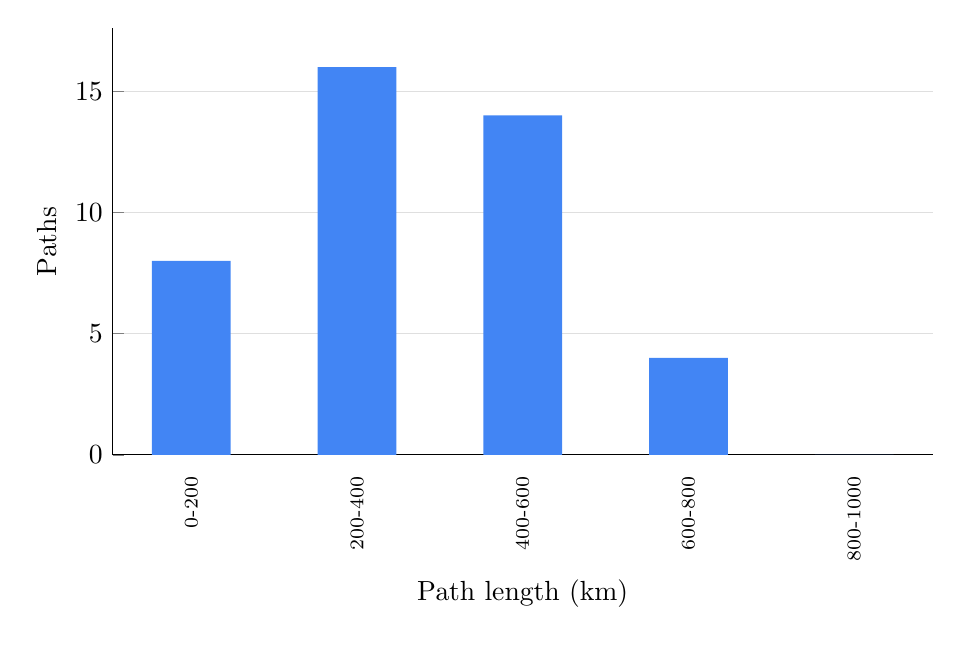
\begin{tikzpicture}
\begin{axis}[
  ybar, bar width=1.000cm, width=12.000cm, height=7cm,
  ymin=0, ymajorgrids, grid style={gray!25}, axis lines*=left,
  enlarge x limits={abs=1.000cm}, xtick=data, major x tick style={draw=none},
  x tick label style={rotate=90, font=\scriptsize, /pgf/number format/1000 sep=},
  legend style={at={(0.5,-0.3)}, anchor=north, legend columns=-1, draw=none},
  ylabel={Paths},
  xlabel={Path length (km)},
  symbolic x coords={0-200,200-400,400-600,600-800,800-1000,1000-1200,1200-1400,1400-1600,1600-1800,1800-2000}]
\addplot[fill={rgb,255:red,66;green,133;blue,244}, draw=none] coordinates {(0-200,8.000) (200-400,16.000) (400-600,14.000) (600-800,4.000) (800-1000,0.000) };
\end{axis}
\end{tikzpicture}\end{center}
\clearpage
\section*{Utilization Entropy}
\begin{center}\begin{adjustbox}{max width=\linewidth}
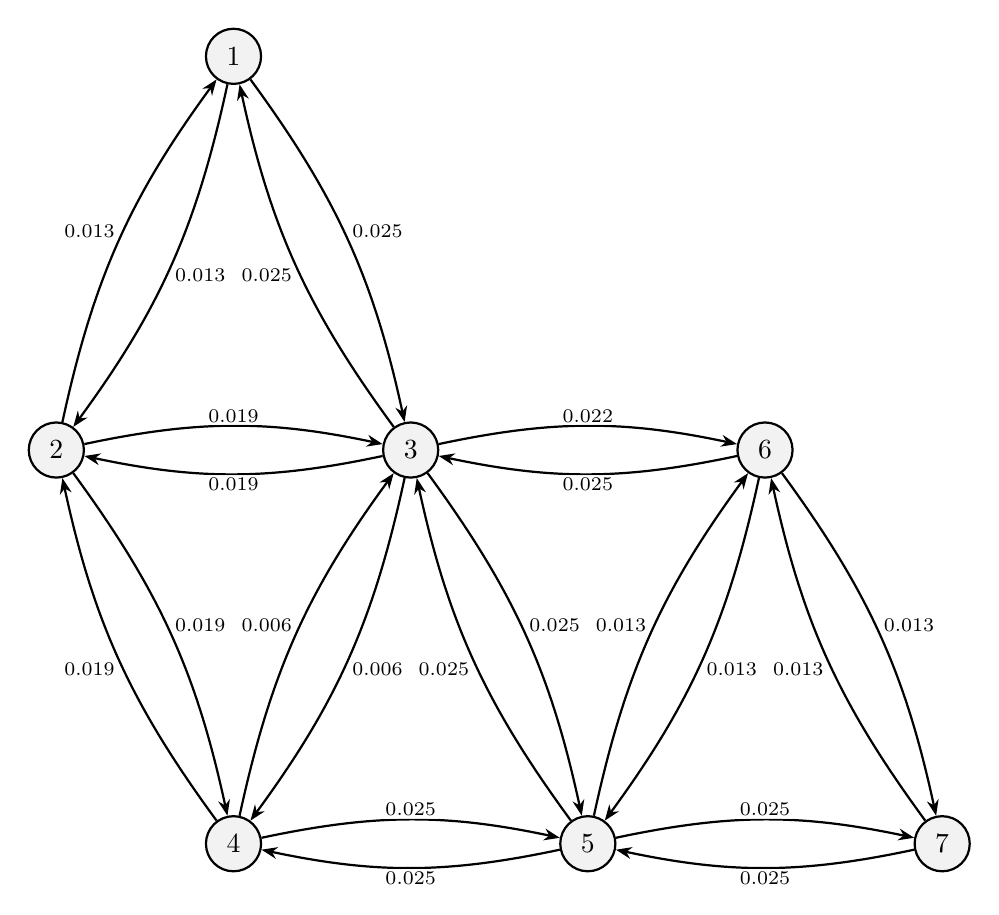
\begin{tikzpicture}[baseline, >={Stealth[length=2mm]},
  netnode/.style={circle, draw, thick, fill=gray!10, minimum size=7mm, inner sep=1pt},
  link/.style={thick},
  linklabel/.style={font=\scriptsize, inner sep=1pt, fill=white, fill opacity=0.85, text opacity=1}]
\node[netnode] (S1) at (2.250,10.000) {1};
\node[netnode] (S2) at (0.000,5.000) {2};
\node[netnode] (S3) at (4.500,5.000) {3};
\node[netnode] (S4) at (2.250,0.000) {4};
\node[netnode] (S5) at (6.750,0.000) {5};
\node[netnode] (S6) at (9.000,5.000) {6};
\node[netnode] (S7) at (11.250,0.000) {7};
\draw[link, ->] (S1) to[bend left=12] node[linklabel, auto] {0.013} (S2);
\draw[link, ->] (S1) to[bend left=12] node[linklabel, auto] {0.025} (S3);
\draw[link, ->] (S2) to[bend left=12] node[linklabel, auto] {0.013} (S1);
\draw[link, ->] (S2) to[bend left=12] node[linklabel, auto] {0.019} (S3);
\draw[link, ->] (S2) to[bend left=12] node[linklabel, auto] {0.019} (S4);
\draw[link, ->] (S3) to[bend left=12] node[linklabel, auto] {0.025} (S1);
\draw[link, ->] (S3) to[bend left=12] node[linklabel, auto] {0.019} (S2);
\draw[link, ->] (S3) to[bend left=12] node[linklabel, auto] {0.006} (S4);
\draw[link, ->] (S3) to[bend left=12] node[linklabel, auto] {0.025} (S5);
\draw[link, ->] (S3) to[bend left=12] node[linklabel, auto] {0.022} (S6);
\draw[link, ->] (S4) to[bend left=12] node[linklabel, auto] {0.019} (S2);
\draw[link, ->] (S4) to[bend left=12] node[linklabel, auto] {0.006} (S3);
\draw[link, ->] (S4) to[bend left=12] node[linklabel, auto] {0.025} (S5);
\draw[link, ->] (S5) to[bend left=12] node[linklabel, auto] {0.025} (S3);
\draw[link, ->] (S5) to[bend left=12] node[linklabel, auto] {0.025} (S4);
\draw[link, ->] (S5) to[bend left=12] node[linklabel, auto] {0.013} (S6);
\draw[link, ->] (S5) to[bend left=12] node[linklabel, auto] {0.025} (S7);
\draw[link, ->] (S6) to[bend left=12] node[linklabel, auto] {0.025} (S3);
\draw[link, ->] (S6) to[bend left=12] node[linklabel, auto] {0.013} (S5);
\draw[link, ->] (S6) to[bend left=12] node[linklabel, auto] {0.013} (S7);
\draw[link, ->] (S7) to[bend left=12] node[linklabel, auto] {0.025} (S5);
\draw[link, ->] (S7) to[bend left=12] node[linklabel, auto] {0.013} (S6);
\end{tikzpicture}
\end{adjustbox}\end{center}

\begin{center}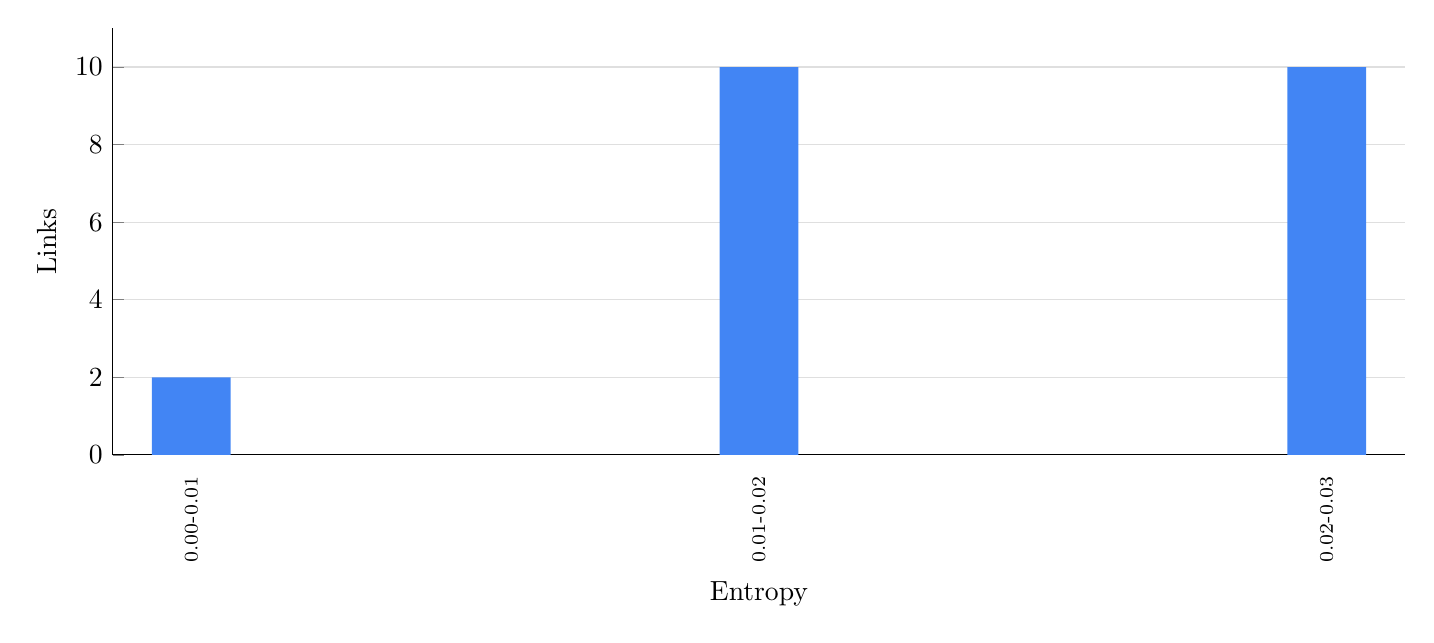
\begin{tikzpicture}
\begin{axis}[
  ybar, bar width=1.000cm, width=18.000cm, height=7cm,
  ymin=0, ymajorgrids, grid style={gray!25}, axis lines*=left,
  enlarge x limits={abs=1.000cm}, xtick=data, major x tick style={draw=none},
  x tick label style={rotate=90, font=\scriptsize, /pgf/number format/1000 sep=},
  legend style={at={(0.5,-0.3)}, anchor=north, legend columns=-1, draw=none},
  ylabel={Links},
  xlabel={Entropy},
  symbolic x coords={0.00-0.01,0.01-0.02,0.02-0.03,0.03-0.04,0.04-0.05,0.05-0.06,0.06-0.07,0.07-0.08,0.08-0.09,0.09-0.10,0.10-0.11,0.11-0.12,0.12-0.13,0.13-0.14,0.14-0.15,0.15-0.16,0.16-0.17,0.17-0.18,0.18-0.19,0.19-0.20,0.20-0.21,0.21-0.22,0.22-0.23,0.23-0.24,0.24-0.25,0.25-0.26,0.26-0.27,0.27-0.28,0.28-0.29,0.29-0.30,0.30-0.31,0.31-0.32,0.32-0.33,0.33-0.34,0.34-0.35,0.35-0.36,0.36-0.37,0.37-0.38,0.38-0.39,0.39-0.40,0.40-0.41,0.41-0.42,0.42-0.43,0.43-0.44,0.44-0.45,0.45-0.46,0.46-0.47,0.47-0.48,0.48-0.49,0.49-0.50,0.50-0.51,0.51-0.52,0.52-0.53,0.53-0.54,0.54-0.55,0.55-0.56,0.56-0.57,0.57-0.58,0.58-0.59,0.59-0.60,0.60-0.61,0.61-0.62,0.62-0.63,0.63-0.64,0.64-0.65,0.65-0.66,0.66-0.67,0.67-0.68,0.68-0.69,0.69-0.70,0.70-0.71,0.71-0.72,0.72-0.73,0.73-0.74,0.74-0.75,0.75-0.76,0.76-0.77,0.77-0.78,0.78-0.79,0.79-0.80,0.80-0.81,0.81-0.82,0.82-0.83,0.83-0.84,0.84-0.85,0.85-0.86,0.86-0.87,0.87-0.88,0.88-0.89,0.89-0.90,0.90-0.91,0.91-0.92,0.92-0.93,0.93-0.94,0.94-0.95,0.95-0.96,0.96-0.97,0.97-0.98,0.98-0.99,0.99-1.00}]
\addplot[fill={rgb,255:red,66;green,133;blue,244}, draw=none] coordinates {(0.00-0.01,2.000) (0.01-0.02,10.000) (0.02-0.03,10.000) };
\end{axis}
\end{tikzpicture}\end{center}
\clearpage
\section*{Shannon Entropy}
\begin{center}\begin{adjustbox}{max width=\linewidth}
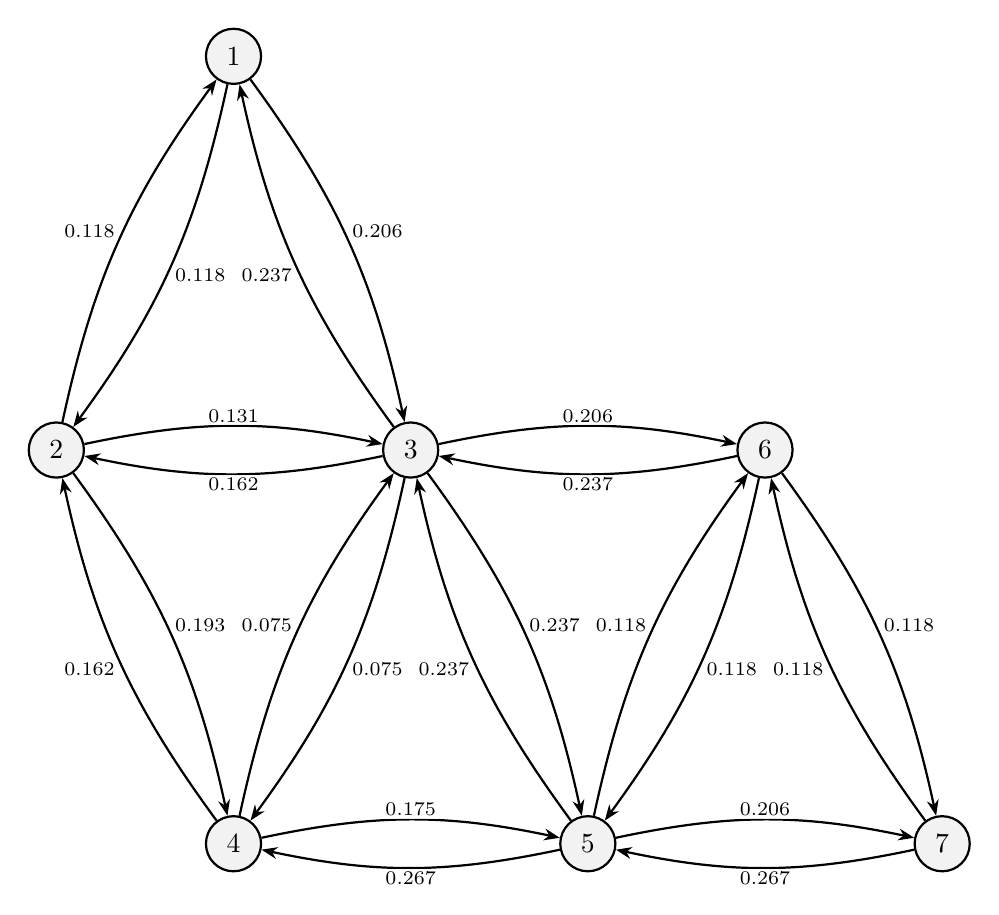
\begin{tikzpicture}[baseline, >={Stealth[length=2mm]},
  netnode/.style={circle, draw, thick, fill=gray!10, minimum size=7mm, inner sep=1pt},
  link/.style={thick},
  linklabel/.style={font=\scriptsize, inner sep=1pt, fill=white, fill opacity=0.85, text opacity=1}]
\node[netnode] (S1) at (2.250,10.000) {1};
\node[netnode] (S2) at (0.000,5.000) {2};
\node[netnode] (S3) at (4.500,5.000) {3};
\node[netnode] (S4) at (2.250,0.000) {4};
\node[netnode] (S5) at (6.750,0.000) {5};
\node[netnode] (S6) at (9.000,5.000) {6};
\node[netnode] (S7) at (11.250,0.000) {7};
\draw[link, ->] (S1) to[bend left=12] node[linklabel, auto] {0.118} (S2);
\draw[link, ->] (S1) to[bend left=12] node[linklabel, auto] {0.206} (S3);
\draw[link, ->] (S2) to[bend left=12] node[linklabel, auto] {0.118} (S1);
\draw[link, ->] (S2) to[bend left=12] node[linklabel, auto] {0.131} (S3);
\draw[link, ->] (S2) to[bend left=12] node[linklabel, auto] {0.193} (S4);
\draw[link, ->] (S3) to[bend left=12] node[linklabel, auto] {0.237} (S1);
\draw[link, ->] (S3) to[bend left=12] node[linklabel, auto] {0.162} (S2);
\draw[link, ->] (S3) to[bend left=12] node[linklabel, auto] {0.075} (S4);
\draw[link, ->] (S3) to[bend left=12] node[linklabel, auto] {0.237} (S5);
\draw[link, ->] (S3) to[bend left=12] node[linklabel, auto] {0.206} (S6);
\draw[link, ->] (S4) to[bend left=12] node[linklabel, auto] {0.162} (S2);
\draw[link, ->] (S4) to[bend left=12] node[linklabel, auto] {0.075} (S3);
\draw[link, ->] (S4) to[bend left=12] node[linklabel, auto] {0.175} (S5);
\draw[link, ->] (S5) to[bend left=12] node[linklabel, auto] {0.237} (S3);
\draw[link, ->] (S5) to[bend left=12] node[linklabel, auto] {0.267} (S4);
\draw[link, ->] (S5) to[bend left=12] node[linklabel, auto] {0.118} (S6);
\draw[link, ->] (S5) to[bend left=12] node[linklabel, auto] {0.206} (S7);
\draw[link, ->] (S6) to[bend left=12] node[linklabel, auto] {0.237} (S3);
\draw[link, ->] (S6) to[bend left=12] node[linklabel, auto] {0.118} (S5);
\draw[link, ->] (S6) to[bend left=12] node[linklabel, auto] {0.118} (S7);
\draw[link, ->] (S7) to[bend left=12] node[linklabel, auto] {0.267} (S5);
\draw[link, ->] (S7) to[bend left=12] node[linklabel, auto] {0.118} (S6);
\end{tikzpicture}
\end{adjustbox}\end{center}

\begin{center}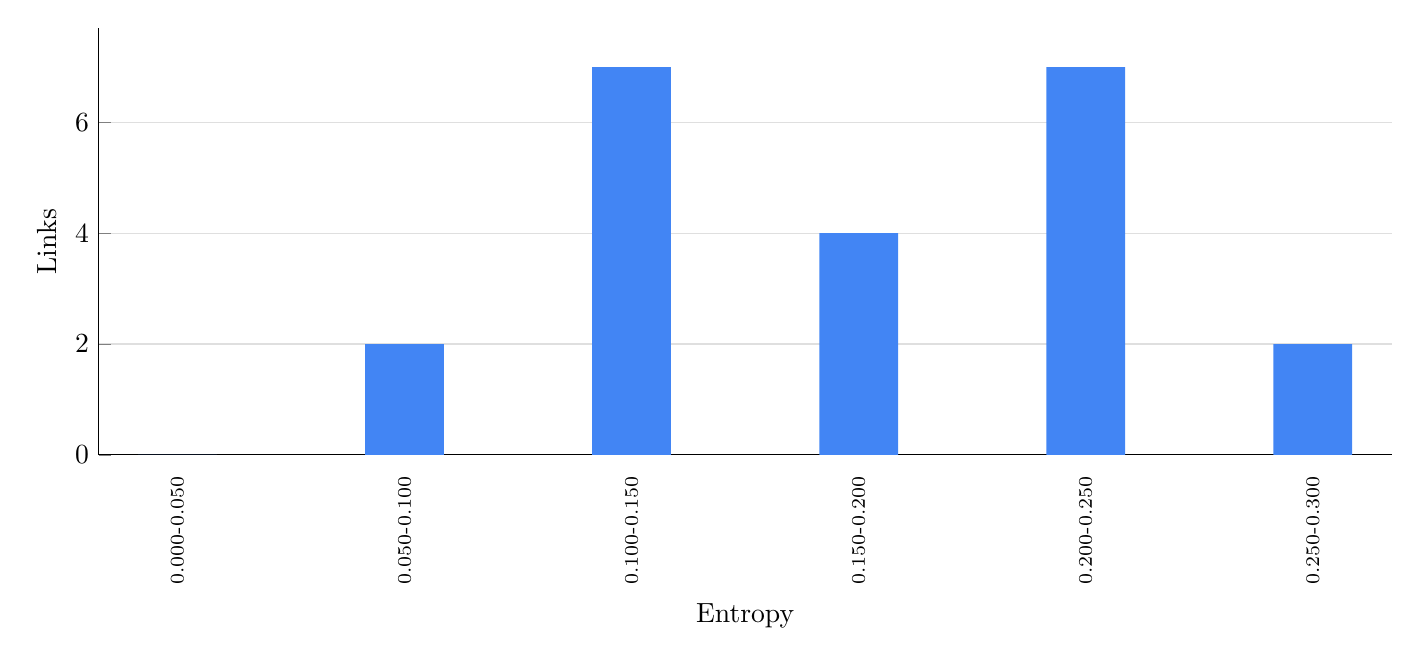
\begin{tikzpicture}
\begin{axis}[
  ybar, bar width=1.000cm, width=18.000cm, height=7cm,
  ymin=0, ymajorgrids, grid style={gray!25}, axis lines*=left,
  enlarge x limits={abs=1.000cm}, xtick=data, major x tick style={draw=none},
  x tick label style={rotate=90, font=\scriptsize, /pgf/number format/1000 sep=},
  legend style={at={(0.5,-0.3)}, anchor=north, legend columns=-1, draw=none},
  ylabel={Links},
  xlabel={Entropy},
  symbolic x coords={0.000-0.050,0.050-0.100,0.100-0.150,0.150-0.200,0.200-0.250,0.250-0.300,0.300-0.350,0.350-0.400,0.400-0.450,0.450-0.500,0.500-0.550,0.550-0.600,0.600-0.650,0.650-0.700,0.700-0.750,0.750-0.800,0.800-0.850,0.850-0.900,0.900-0.950,0.950-1.000}]
\addplot[fill={rgb,255:red,66;green,133;blue,244}, draw=none] coordinates {(0.000-0.050,0.000) (0.050-0.100,2.000) (0.100-0.150,7.000) (0.150-0.200,4.000) (0.200-0.250,7.000) (0.250-0.300,2.000) };
\end{axis}
\end{tikzpicture}\end{center}

\end{document}
